\documentclass[a4paper, 12pt]{article}

\usepackage[utf8]{inputenc}
\usepackage[spanish]{babel}
\usepackage[T1]{fontenc}
\usepackage{fancyhdr}
\usepackage{graphicx}
\usepackage{listings}
\usepackage{minted}
\usepackage[a4paper, total={6in, 8in}]{geometry}
\usepackage[ruled,vlined]{algorithm2e}
\usepackage[toc,page]{appendix}

\pagestyle{fancy}
\fancyhf{}
\rhead{Martín Romera Sobrado}
\chead{EPED}
\lhead{PEC}
\cfoot{\thepage}

\begin{document}
    
    \begin{titlepage}
        
        \centering
		\vspace*{1cm}
		
		\Huge
		\textbf{Estrategias de Programación y Estructuras de Datos}\\
		\textbf{PEC - 2021}
		
		\vspace{0.5cm}
		\LARGE
		Centro Asociado de la UNED en Bizkaia\\
		\vspace{1.5cm}
		
		\textbf{Martín Romera Sobrado}\\
		\textbf{Bilbao}
		
		\vfill
		
		\vspace{0.8cm}
		\Large
		\today

    \end{titlepage}

    \section{Preguntas teóricas}

        \subsection{Bucket Queue}

            \subsubsection{Pregunta 1 : Secuencia adecuada}

                \textit{¿Qué tipo de secuencia sería la adecuada para realizar 
                esta implementación? ¿Por qué? ¿Qué consecuencias tendría el
                uso de de otro tipo de secuencias?}\\\mbox{}

                La opción más viable sería implementarlo sobre una lista, ya que
                el orden de la secuencia \texttt{SamePriorityQueue} no está 
                por el orden de entrada de estas en la \texttt{BucketQueue}. Las 
                pilas y colas tienen un orden definido por el orden de entrada, 
                lo cual las hace inconvenientes, sin embargo en la lista podemos
                alterar su orden a nuestro gusto, en este caso por la propiedad
                \texttt{priority} de las propias \texttt{SamePriorityQueue}.
            
            \subsubsection{Pregunta 2 : Funcionamiento de operaciones}

                \textit{Describe el funcionamiento de las operaciones 
                \texttt{getFirst}, \texttt{enqueue} y \texttt{dequeue} con esta
                estructura de datos.}\\\mbox{}

                \begin{itemize}
                    \item \texttt{getFirst} : Se encargará de obtener el primer 
                    elemento en la cola de prioridad, de forma que accedera a la 
                    priemra \texttt{SamePriorityQueue} de la lista y obtendrá su
                    primer elemento mediante \texttt{getFirst}.
                    \item \texttt{enqueue} : Se encargará de encolar el elemento
                    en su \texttt{SamePriorityQueue} correspondiente, de forma 
                    que irá recorriendo la lista hasta que encuentre una 
                    \texttt{SamePriorityQueue} con mismo o menor valor de 
                    prioridad. Si encuentra una \texttt{SamePriorityQueue} con 
                    misma prioridad que el elemento entonces lo encola en esa 
                    misma cola. Si la cola que encuentra tiene menor prioridad,
                    entonces crea una \texttt{SamePriorityQueue} nueva con el 
                    elemento y la inserta en la lista antes de la cola con menor
                    prioridad que hemos encontrado en la busqueda. Si no 
                    encuentra ninguna \texttt{SamePriorityQueue} con menor o 
                    igual prioridad entonces, crea una nueva cola con el 
                    elemento y la inserta al final de la cola.
                    \item \texttt{dequeue} : Se encargará de extraer el elemento
                    en la cabeza de la cola de prioridad. Para eso extraerá el 
                    primer elemento de la \texttt{SamePriorityQueue} de la 
                    lista. Si con esa acción la \texttt{SamePriorityQueue} se 
                    queda vacía (\texttt{isEmpty()}) entonces la eliminará de 
                    la lista dejando ahora en primera posición a la siguiente 
                    cola con menor prioridad.
                \end{itemize}

            \subsubsection{Pregunta 3 : Funcionamiento del iterador}

                \textit{Describe el funcionamiento del iterador de la cola con 
                piroridad en esta implementación.}\\\mbox{}

                El iterador iterará sobre cada elemento del \texttt{BucketQueue}
                para ello podemos hacer uso de los iteradores de la
                implementación de \texttt{List} (\texttt{listIterator}) y de la
                implementación de \texttt{SamePriorityQueue} 
                (\texttt{subIterator}). \texttt{listIterator} iterará sobre las
                \texttt{SamePriorityQueue} de la lista y \texttt{subIterator} 
                iterará sobre los elementos de las \texttt{SamePriorityQueue} a 
                las que apunta \texttt{listIterator}. Devolveremos el valor al 
                que apunta en cada momento el \texttt{subIterator}, y 
                actualizaremos la \texttt{SamePriorityQueue} sobre la que itera 
                cada vez que se quede sin elementos en la anterior 
                (\texttt{!hasNext()}) con ayuda de \texttt{listIterator}.

        \subsection{Árbol Binario de Busqueda}

            \subsubsection{Pregunta 1 : Funcionamiento de las operaciones}

                \textit{Describe el funcionamiento de las operaciones 
                \texttt{getFirst}, \texttt{enqueue} y \texttt{dequeue} con esta
                estructura de datos.}\\\mbox{}

                \begin{itemize}
                    \item \texttt{getFirst} : Esta operación se aprovecha del
                    iterador, creando uno para el objeto 
                    \texttt{BSTPriorityQueue} y obteniendo el primer elemento
                    con \texttt{getNext}. \\\mbox{}
                    \item \texttt{enqueue} : También se aprovecha del iterador 
                    de la clase \texttt{BSTPriorityQueue}. Recorre con el
                    iterador todo el árbol comprobando si hay algún nodo con una 
                    \texttt{SamePriorityQueue} con la misma prioridad que el 
                    elemento en la que encolarlo. Si lo encuentra lo encola en 
                    esa misma cola y si no, crea una nueva 
                    \texttt{SamePriorityQueue}, encola el elemento y lo añade 
                    al árbol con el método nativo \texttt{add} de la clase 
                    \texttt{BSTree} que lo añade en su posición correcta del
                    árbol.
                    \item \texttt{dequeue} : De nuevo nos aprovechamos del
                    iterador para apuntar al elemento con mayor prioridad 
                    llamando una sola vez a \texttt{getNext} y hacemos un 
                    \texttt{dequeue} del resultado.
                \end{itemize}

            \subsubsection{Pregunta 2 : Funcionamiento del iterador}

                \textit{Describe el funcionamiento de la cola con prioridad en 
                esta implementación}\\\mbox{}

                El iterador hará uso de dos iteradores. Uno de ellos
                (llamemoslo \texttt{treeIterator}) iterará sobre los diferentes
                nodos del árbol apuntando en cada iteración a una nueva 
                \texttt{SamePriorityQueue}. El otro iterador (llamemoslo 
                \texttt{subIterator}) iterará sobre los elementos contenidos por
                la \texttt{SamePriorityQueue} a la que apunta 
                \texttt{treeIterator}. Cuando \texttt{subIterator} no tenga nada
                más que recorrer, actualizamos \texttt{treeIterator} al
                siguiente nodo y hacemos que \texttt{subIterator} sea el 
                iterador de esta nueva \texttt{SamePriorityQueue}.

        \subsection{Estudio empírico del coste}

            \subsubsection{Cálculo del coste asintótico temporal}

                \textit{Calcule el coste asintótico temporal en el caso peor de
                las operaciones \texttt{enqueue} y \texttt{dequeue} para ambas
                implementaciones}.\\\mbox{}

                Para la implementación de \texttt{BucketQueue} la operación
                \texttt{enqueue} funciona como si encolaramos en una 
                \texttt{Queue} contenida en la $n$-sima posición de una 
                \texttt{List}. Esta operación tiene un coste lineal $O(n)$.
                Por otra parte la función \texttt{dequeue} tendrá siempre un 
                coste constante, ya que para desencolar el elemento de mayor 
                prioridad este se encontrará en la cabeza de la cola en la
                primera posición siempre. Acceder al elemento $n$ de una lista 
                tiene un coste de $O(n)$, como $n=1$ es una constante, entonces 
                el tiempo de ejecución también $O(1)$ y desencolar elementos de
                una cola también tiene un tiempo de ejecución constante $O(1)$ 
                de lo que observamos que esta operación tiene un tiempo de 
                ejecuión constante.
                \\\mbox{}

                Para la implementación de \texttt{BSTPriorityQueue} sin embargo
                las operaciones tendrán un coste acorde a la profundiad del 
                árbol que contenga las colas ($h$ a partir de ahora). Esto tiene 
                sus ventajas y desventajas. La ventaja es que un árbol binario 
                de busqueda equilibrado tendrá una proundidad logarítmica 
                respecto al número de elementos ($n$), es decir $h = \log_2 n$. 
                Sin embargo si el árbol no está balanceado $h$ estará 
                en un valor entre $\log_2 n$ y $n$. En el peor caso $h$ será $n$,
                haciendo que la estructura tenga semejanza a una lista como la 
                que usa \texttt{BucketQueue} y por ende los costes temporales de 
                sus operaciones serán iguales, $O(n)$ para \texttt{enqueue} y 
                $O(1)$ para \texttt{dequeue}. Por supuesto \texttt{enqueue} no 
                tendrá siempre un coste lineal, a que su coste dependerá de $h$,
                de forma que realmente el coste de esta operación realmente es 
                $O(h)$.\\\mbox{}

            \subsubsection{Comparación entre coste asintótico y costes empíricos}

                \textit{Compare el coste asintótico temporal obtenido en la 
                pregunta anterior con los costes empíricos obtenidos. ¿Coincide
                el coste calculado con el coste real?}
                \\\mbox{}

                Para probar los algoritmos se realizan 6 pruebas sobre cada 
                función, cada una estructura de 1000, 2000, 3000, 4000, 5000 o 
                6000 nodos con colas de un solo elemento, cada test se ejecutará
                500 veces. Las colas solo tienen un elemento ya que no nos 
                interesa evaluar el \texttt{enqueue} o \texttt{dequeue} de 
                \texttt{SamePriorityQueue} si no el de las estructuras 
                \texttt{BucketQueue} y \texttt{BSTPriorityQueue}. \\\mbox{}
                
                Para \texttt{BucketQueue} la operación \texttt{enqueue} los
                tests nos dan los resultados de la figura \ref{f:enq_bq_test}.
                \\\mbox{}

                \begin{figure}[ht!]
                    \centering
                    \begin{tabular}{|c|c|c|}
                        \hline
                        \textbf{Número de nodos} & \textbf{$\sigma_t$}  & \textbf{$t$} \\\hline
                        $1000$                   & $2.927029$           & $22.35$        \\\hline
                        $2000$                   & $4.635256$           & $55.12$        \\\hline
                        $3000$                   & $5.282755$           & $107.65$       \\\hline
                        $4000$                   & $17.580384$           & $192.51$       \\\hline
                        $5000$                   & $8.428968$           & $294.45$        \\\hline
                        $6000$                   & $13.587877$          & $407.36$       \\\hline                  
                    \end{tabular}
                    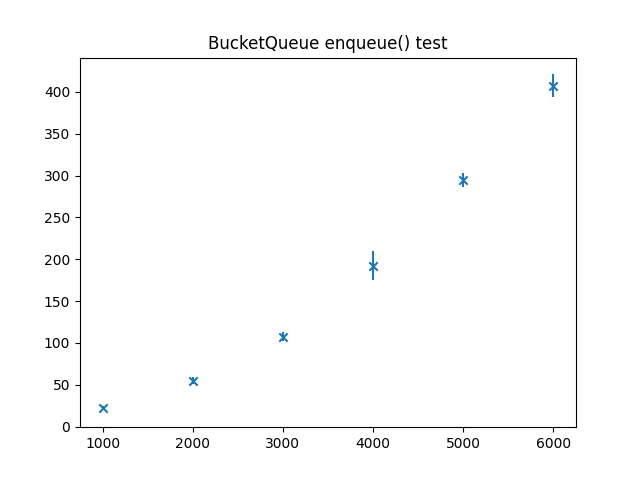
\includegraphics[]{img/costemp_bq_enq.png}
                    \caption{Resultados del test de coste empírico para 
                    \texttt{enqueue} de \texttt{BucketQueue}}
                    \label{f:enq_bq_test}
                \end{figure}

                El resultado del test empírico no es completamente lineal, esto 
                puede deberse principalmente a el margen de error del tiempo de 
                ejecución ($\sigma_t$), que vemos que también incrementa con el 
                tiempo (exceptuando el 4º caso que por algún motivo tiene un
                margen de error de tiempo mayor, tal vez por las cosas que había
                en ejecución en ese momento en mi ordenador). De todas formas la 
                forma que adopta el resultado del test es casí lineal.
                \\\mbox{}
                La operación \texttt{dequeue} dijimos que tenía un tiempo de 
                ejecución constante, y el resultado del test lo muestra más o 
                menos, como podemos ver en la figura 
                \ref{f:deq_bq_test}.\\\mbox{}

                \begin{figure}[ht!]
                    \centering
                    \begin{tabular}{|c|c|c|c|c|}
                        \hline
                        \textbf{Número de nodos} & \textbf{$\sigma'$} & \textbf{$|\sigma|$} & \textbf{$t'$}    & \textbf{$t$}      \\\hline
                        $1000$                   & $1.905020$         & $1,022009$          & $21.47$         & $-0.88$        \\\hline
                        $2000$                   & $3.364209$         & $1.271047$         & $55.89$         & $0.86$        \\\hline
                        $3000$                   & $3.602999$         & $1.679756$           & $116.28$        & $8.63$       \\\hline
                        $4000$                   & $8.867604$         & $8.71278$          & $189.16$        & $-3.35$       \\\hline
                        $5000$                   & $8.098173$         & $0.330795$         & $292.14$        & $-2.31$        \\\hline
                        $6000$                   & $14.510341$        & $0.922464$          & $407.70$        & $-0.34$       \\\hline                  
                    \end{tabular}
                    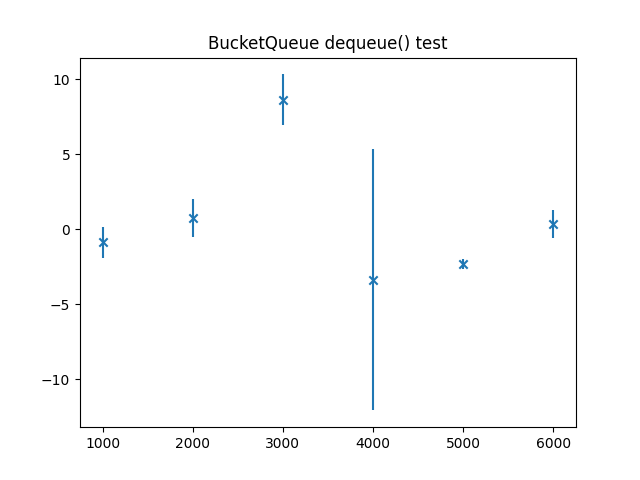
\includegraphics[]{img/costemp_bq_deq.png}
                    \caption{Resultados del test de coste empírico para 
                    \texttt{dequeue} de \texttt{BucketQueue}}
                    \label{f:deq_bq_test}
                \end{figure}

                Para este test lo que se ha hecho es restar el resultado de 
                tiempo de este test, con el resultado del caso correspondiente 
                en el test anterior (para restar el tiempo de encolar todos los
                elementos). Como puede observarse, la tendencia de tiempo 
                no es creciente en ningún momento, fluctua entre los tests cerca
                de los 0 ms lo que denota una tendencia de tiempo constante.
                \\\mbox{}

                Vamos ahora con \texttt{BSTPriorityQueue}, analizamos primero la 
                operación \texttt{enqueue} y obtenemos los resultados de la 
                figura \ref{f:enq_bst_test}.

                \begin{figure}[ht!]
                    \centering
                    \begin{tabular}{|c|c|c|}
                        \hline
                        \textbf{Número de nodos} & \textbf{$\sigma_t$}  & \textbf{$t$} \\\hline
                        $1000$                   & $3.594704$           & $21.91$        \\\hline
                        $2000$                   & $3.403219$           & $56.41$        \\\hline
                        $3000$                   & $4.908146$           & $118.01$       \\\hline
                        $4000$                   & $9.459783$           & $189.95$       \\\hline
                        $5000$                   & $9.056401$           & $295.04$        \\\hline
                        $6000$                   & $15.672090$          & $408.16$       \\\hline                  
                    \end{tabular}
                    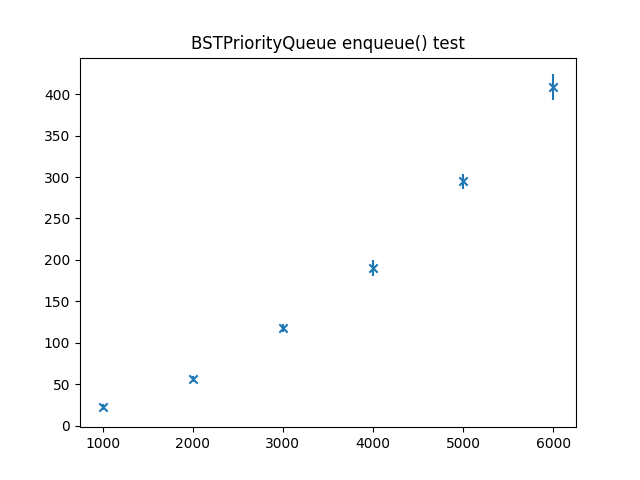
\includegraphics[]{img/costemp_bst_enq.png}
                    \caption{Resultados del test de coste empírico para 
                    \texttt{enqueue} de \texttt{BSTPriorityQueue}}
                    \label{f:enq_bst_test}
                \end{figure}

                De nuevo, el resultado no es completamente lineal, pero vemos
                que tiene una tendencia similar al test de la operación 
                \texttt{enqueue} de la anterior implementación. Esto es porque 
                esta estructura en el caso peor tiene la misma forma que una 
                lista enlazada, de forma que el tiempo de ejecución de 
                \texttt{enqueue} es lineal (o casí lineal prácticamente) y el 
                tiempo de \texttt{dequeue} constante como podemos ver en la 
                tendencia que muestra \ref{f:deq_bst_test}.
                

                \begin{figure}[ht!]
                    \centering
                    \begin{tabular}{|c|c|c|c|c|}
                        \hline
                        \textbf{Número de nodos} & \textbf{$\sigma'$} & \textbf{$|\sigma|$} & \textbf{$t'$}    & \textbf{$t$}      \\\hline
                        $1000$                   & $1.894624$         & $1,70008$          & $21.48$         & $0.43$        \\\hline
                        $2000$                   & $2.946184$         & $0.457035$         & $57.00$         & $-0.59$        \\\hline
                        $3000$                   & $3.255530$         & $1.652616$          & $116.94$        & $-1.07$       \\\hline
                        $4000$                   & $9.026073$         & $0.43371$          & $189.70$        & $-0.25$       \\\hline
                        $5000$                   & $6.277866$         & $2.778535$         & $292.22$        & $-2.82$        \\\hline
                        $6000$                   & $26.366454$        & $10.694364$          & $412.01$        & $3.85$       \\\hline                  
                    \end{tabular}
                    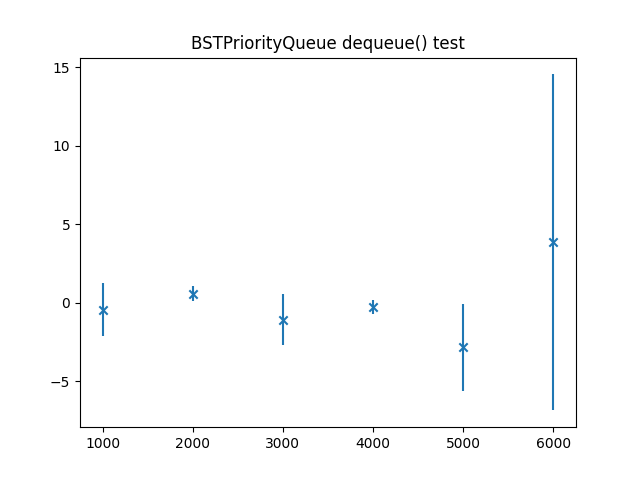
\includegraphics[]{img/costemp_bst_deq.png}
                    \caption{Resultados del test de coste empírico para 
                    \texttt{dequeue} de \texttt{BSTPriorityQueue}}
                    \label{f:deq_bst_test}
                \end{figure}
              
\end{document}